For a sensor network the routing protocol used for transmitting data from motes to
the base station plays an important role because sensors' resources are limited and 
and their lifetime could be drasticaly reduced if not using an appropriate protocol.
A straight-forward solution could be to use a direct communication protocol where
each sensor sends its data to the base station directly but sending data over a 
long distance is a very energy consuming operation, much expensive than a series
of local computations.
In the following section we present a short description of LEACH, a routing protocol for sensor networks, and
its implementation in TOSSIM and ns-2 simulators along with some conclusions regarding 
these two simulators based on the compararison of the behaviour and results of the same protocol.  


\subsection{ Short routing protocol description}
LEACH\cite{leach-desc}(Low-Energy Adaptive Clustering Hierarchy) is a clustering-based protocol
that minimizes energy disipation in sensor networks. Its main characteristics are that
it uses localized coordination and control for cluster set-up and operation, it
rotates the "cluster-head" nodes in order to evenly distribute energy consumption and
it uses local compression of data so that global communication (and bandwidth)
is reduced.
The nodes organize in local clusters with one node being elected the cluster-head; it is randomly chosen
and it is cluster-head just for a limited amount of time. The election of cluster head
is based on a priority each of the motes has, which is computed based on the energy
each mote has.

The LEACH algorithm is broken up into rounds which begin with a set-up phase when organizing the 
network and selecting the cluster head and a steady-state phase when data is being transmitted.
In the advertisment phase a node decides whether to become a cluster-head or not based
on the suggested percentage of cluster heads for the network which is chisen a priori (based
on the network size and other factors) and on the number of times it has already been a cluster-head. 
Each node generates a random number between 0 and 1. If this number is less than a threshold value the node becomes cluster
head for the curremt round. After electing itself a cluster-heads  a node broadcasts a 
message to the rest of the nodes. During the first phase each non-cluster-head node keeps its receivers on.
When the advertisment phase it is over each non-cluster-head node decides in which
cluster to be in this round. This decision is based on the signal strenght of the received advertising
messages.
After choosing a cluster, each non-cluster-head node sends a message
to the cluster-head corresponding to that cluster which, after receiving these messages
creates a TDMA\cite{tdma} schedule telling each node when it can transmit data and it broadcasts
this to the nodes in the cluster.
After this, data transmition begins which lasts for a predefined amount of time and afterwards a next
round begins having the same phases.

 
%%say about the article and energy measurements

\subsection{Simplifications and assumptions used in our implementation}
A full LEACH implementation was not neccessary because only some caracteristics of
the simulators where observed. Instead of having more rounds and changing the topology
so that the nodes don't run out of energy, the topology is only calculated once after
which only data traffic is present.
\subsection{TOSSIM implementation}
TOSSIM is really easy to get used to when first working with it. There are many examples
available, from simple ones to more complex. The user is in control of everything that is
run on the node and not much is hidden from him.

\subsection{ns-2 implementation}
NS2 has abstractions for every possible layer. Even though a user would normally not need to use
all of these abstractions, they would have a hard time finding what they need to use through all 
the classes.

\subsection{Tests}
\begin{itemize}
    \item{CPU utilization}
	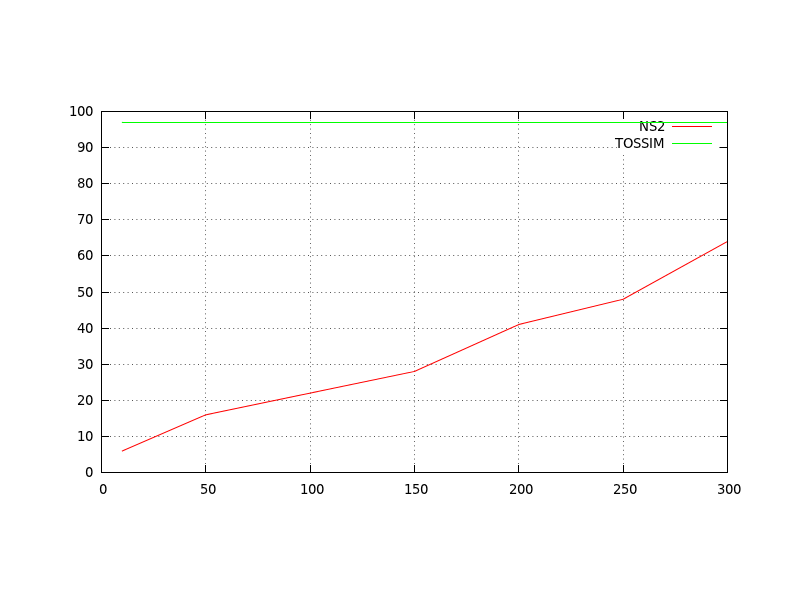
\includegraphics[scale=0.35]{img/cpu.png}
    \item{Memory}
	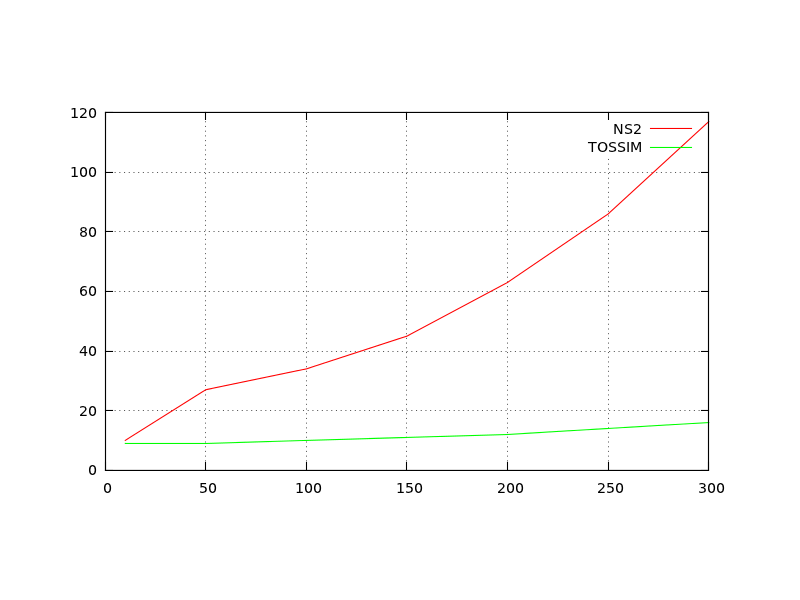
\includegraphics[scale=0.35]{img/mem.png}
\end{itemize}
